\subsection{UNISA}

%En este experimento decidimos realizar el traceroute hacia la universidad de UNISA, ubicada en Sudáfrica. Para la realización del mismo decidimos establecer un $TTL\_MAX$ de 30 saltos, es decir que cortabamos la ejecución si no alcanzabamos el destino en, a lo sumo, 30 saltos. Por otro lado, por cada iteración de los $TTL$ emitimos una ráfaga de 30 paquetes.

Comencemos por describir la ruta generada:
Se han realizado 27 saltos hasta alcanzar el destino solicitado, de los cuales en el $85 \% $ de los mismos aproximadamente, hemos obtenido respuestas del tipo $TIME\_EXCEEDED$, determinando así que el largo de nuestra ruta es de 23 saltos, y que del resto de los valores del $TTL$ no hemos obtenido respuesta alguna. Como también se puede ver en la figura \ref{mapa-unisa}, y en el cuadro \ref{tabla-unisa}, durante el trayecto se realizaron 4 saltos intercontinentales. Por otra parte, el método de Cimbala nos ha detectado en un principio todo número positivo como outlier, pero al sacar los 0s sólo ha detectado aquellos que se muestran en el cuadro ya mencionado.

\begin{table}[!htbp]
\centering
\caption{My caption}
\label{tabla-unisa}
\begin{tabular}{|c|c|c|c|}
\hline
\textbf{TTL} & \textbf{IP}    & \textbf{COUNTRY} & \textbf{OUTLIERS} \\ \hline
1   & 10.0.2.2       & Undefined      &               \\ \hline
6   & 200.89.161.129 & Argentina      & {[}outlier{]} \\ \hline
7   & 200.89.165.5   & Argentina      &               \\ \hline
8   & 200.89.165.250 & Argentina      &               \\ \hline
9   & 195.22.220.102 & Italy          &               \\ \hline
10  & 89.221.41.187  & United States  & {[}outlier{]} \\ \hline
11  & 89.221.41.187  & United States  &               \\ \hline
12  & 154.54.9.17    & United States  & {[}outlier{]} \\ \hline
13  & 154.54.80.41   & United States  &               \\ \hline
14  & 154.54.24.193  & United States  &               \\ \hline
15  & 154.54.7.157   & United States  & {[}outlier{]} \\ \hline
16  & 154.54.40.105  & United States  &               \\ \hline
17  & 154.54.30.186  & United Kingdom & {[}outlier{]} \\ \hline
18  & 154.54.58.174  & United Kingdom &               \\ \hline
19  & 154.54.56.242  & United Kingdom &               \\ \hline
20  & 149.14.80.210  & United Kingdom & {[}outlier{]} \\ \hline
21  & 196.32.209.174 & South Africa   & {[}outlier{]} \\ \hline
22  & 155.232.6.65   & South Africa   & {[}outlier{]} \\ \hline
23  & 155.232.6.37   & South Africa   &               \\ \hline
24  & 155.232.6.33   & South Africa   &               \\ \hline
25  & 155.232.6.142  & South Africa   &               \\ \hline
26  & 155.232.6.145  & South Africa   & {[}outlier{]} \\ \hline
27  & 155.232.6.138  & South Africa   &               \\ \hline
\end{tabular}
\end{table}

\newpage

\begin{figure}[!htbp]
  \centering
    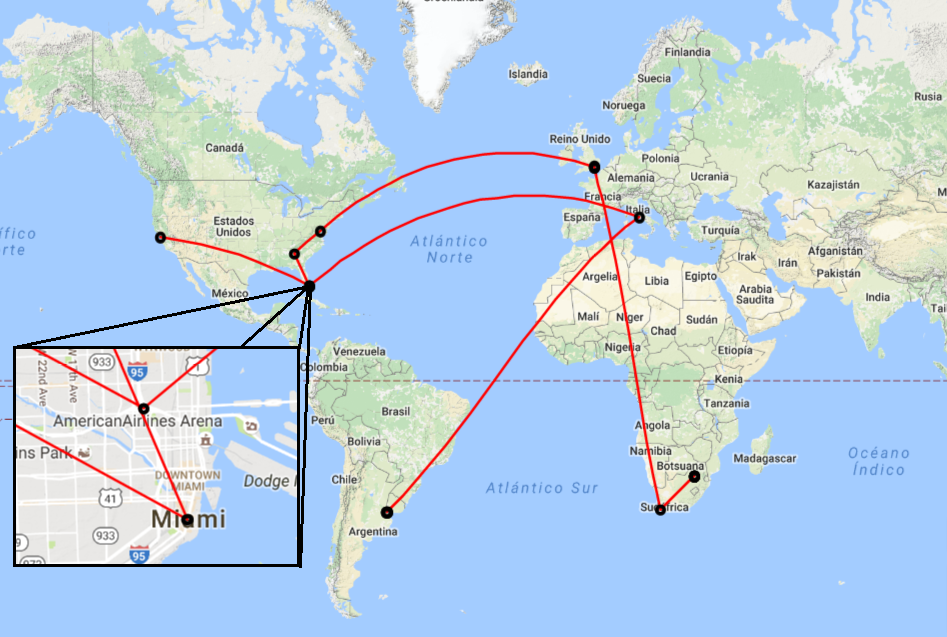
\includegraphics[scale=0.6]{imagenes/unisa-graficos/mapa-unisa.png}
  \caption{UNISA- RTT hops}
  \label{mapa-unisa}
\end{figure}

En este contexto, nos disponemos a realizar un análisis más profundo de nuestros resultados. Podemos observar entonces, que de los cuatro saltos intercontinentales, Cimbala identifica correctamente todos, salvo el de Argentina a Italia, cuestión que podemos atribuirle a que, como muestra la figura \ref{fig:1}, el rtt de ese salto es 0. Por otro lado, 
 aunque identifica un par de saltos más, produciendo falsos positivos. Como se puede observar en la figura \ref{fig:1} los rtts correspondientes correspondientes a los saltos continentales tienen un valor claramente más elevado que el resto, con la excepción del primer salto, que tiene un rtt de 20 ms aproximadamente, numero no mayor al ttl 26 que no es un salto continental. Podríamos inferir que esta anomalía es la causante de que Cimbala identifique al ttl 26 como intercontinental cuando no lo es, pero esto

Al realizar el experimento, se logró llegar al destino en el ttl 27. De estos, 4 no respondieron. Los ttls que Cimbala reconoció como intercontinentales fueron 6, 10, 12, 15, 17, 20, 21, 22 y 26.

\begin{figure}[!htbp]
  \centering
    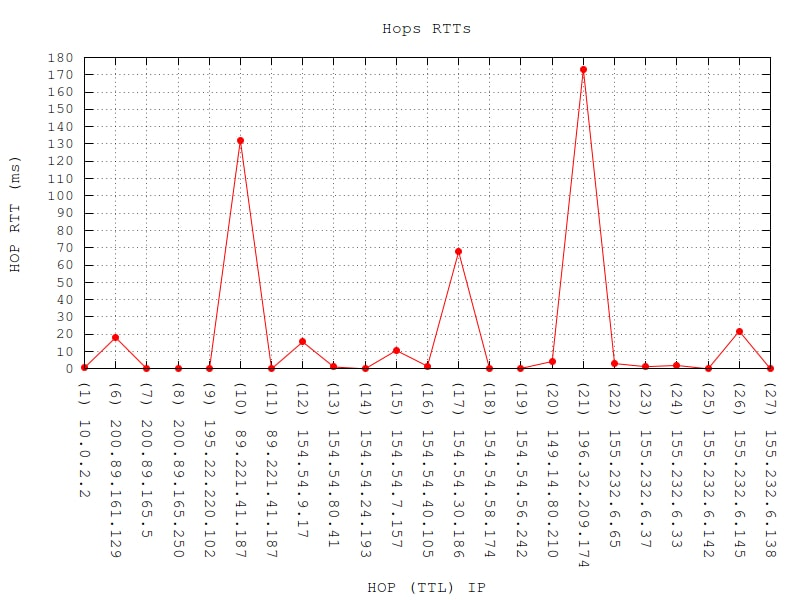
\includegraphics[scale=0.6]{imagenes/unisa-graficos/traceroute-unisa.jpg}
  \caption{UNISA- RTT hops}
  \label{fig:1}
\end{figure}

En la figura \ref{fig:1} se puede observar como el ttl 10, 17 y 21 tienen un rtt claramente distinguido del resto.

\begin{figure}[!htbp]
  \centering
    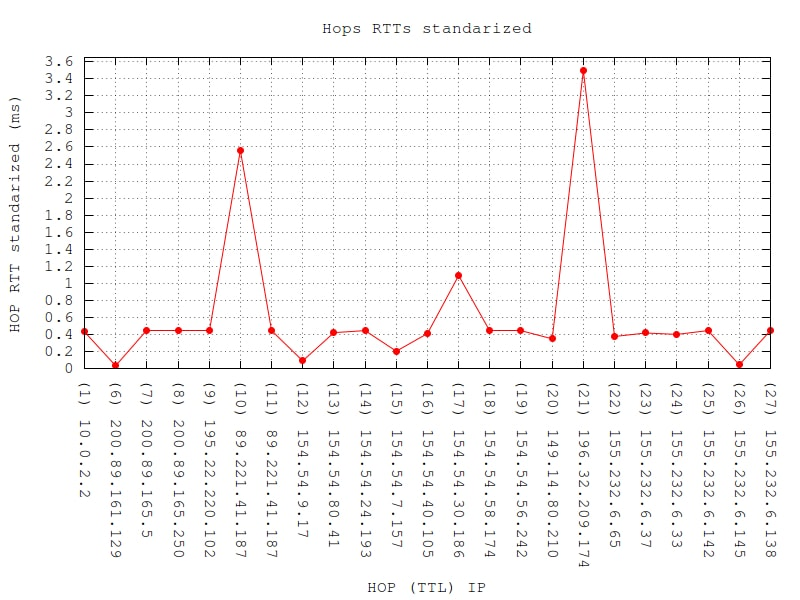
\includegraphics[scale=0.6]{imagenes/unisa-graficos/traceroute-unisa-standarized.jpg}
  \caption{UNISA- RTT hops standarized}
  \label{fig:2}
\end{figure}

En la figura \ref{fig:2} se puede observar una situacion similar a la de la figura \ref{fig:1}.

